
%Chapter without numbering on page, but still added to ToC
\chapter*{ChapterName}
\setcounter{chapter}{1}
\setcounter{section}{0}
\addcontentsline{toc}{chapter}{\protect\numberline{}ChapterName}
\thispagestyle{fancy} %Using fancyheader
\label{ch:ChapterReference}
%%%%%%%%%%%%%%%%%%%%%%%%%%%%%%%%%%%%%%%%%%

%Bullet list
\begin{itemize}
    \item sampling frekvens: $f_s$ = \FS 
    \item 3 dB båndbredde: BW = 25 Hz
    \item Center frekvens: $f_0$ = 50 Hz
\end{itemize}
%%%%%%%%%%%%%%%%%%%%%%%%%%%%%%%%%%%%%%%%%%

%Equation
\begin{equation}
    r = 1 -\bigg(\frac{BW_{3dB}}{f_s}\bigg)\cdot\pi \implies
    1-\bigg(\frac{\SI{25}{\hertz}}{\FS}\bigg)\cdot\pi = 0.9964381036
\end{equation}
%%%%%%%%%%%%%%%%%%%%%%%%%%%%%%%%%%%%%%%%%%

%Insert image
\begin{figure}[H]%[H] requires the float package, standard options are [htb!]
\center
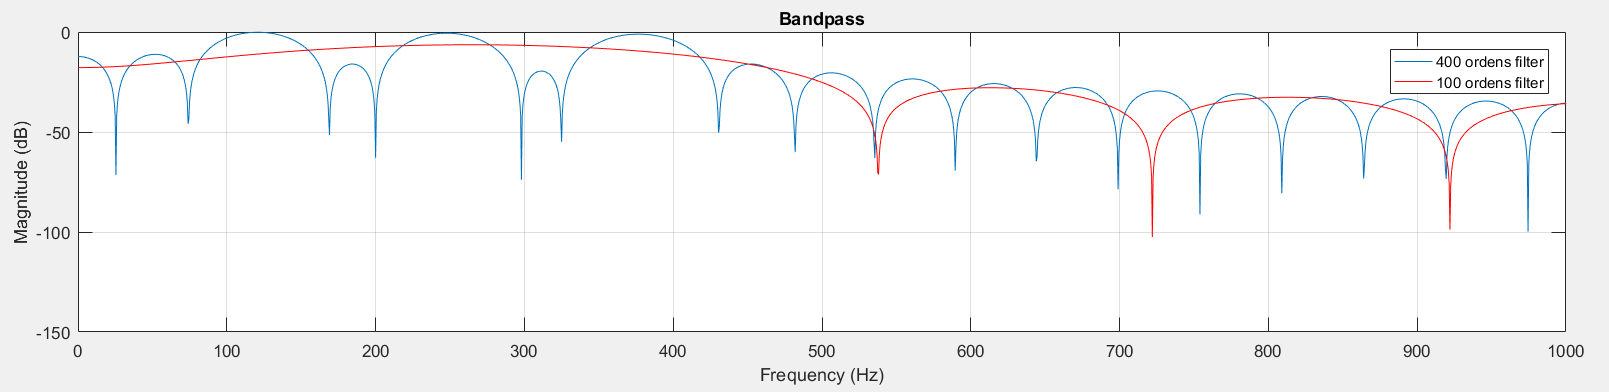
\includegraphics[scale=0.7]{NameOfImage}
\caption{Caption text goes here}
\label{fig:Reference}
\end{figure}
%%%%%%%%%%%%%%%%%%%%%%%%%%%%%%%%%%%%%%%%%%

%Aligned equations
\begin{align}
   f_h = f_0 + \frac{W_{pass}}{2} &\implies \SI{50}{\hertz} + \frac{\SI{50}{\hertz}}{2} = \SI{75}{\hertz}\\
   f_l = f_0 + \frac{W_{pass}}{2} &\implies \SI{50}{\hertz} - \frac{\SI{50}{\hertz}}{2} = \SI{25}{\hertz}\\
   T=\frac{1}{f_s} &\implies \frac{1}{\FS}
\end{align}
%%%%%%%%%%%%%%%%%%%%%%%%%%%%%%%%%%%%%%%%%%

\begin{equation}
\begin{aligned}
  &\omega_{ah} = \frac{2}{T}*tan\bigg(\frac{\omega_h*T}{2}\bigg) \implies\\ &44100*tan\bigg(\frac{150*\pi/\FS}{2}\bigg) = \SI{471.2568349}{\radian\per\second}
  \end{aligned}
\end{equation}

%Math in text
Der vælges $\omega_{ah}=\SI{471.2568349}{\radian\per\second},\ \omega_{al}=\SI{209.4386244}{\radian\per\second},\ \omega_{sh}=\SI{392.7094616}{\radian\per\second}$ og $\omega_{sl}=\SI{251.3292724}{\radian\per\second}$ for at få den smalleste bredde, så der fjernes så lidt muligt af frekvenserne tæt ved 50 Hz.
%%%%%%%%%%%%%%%%%%%%%%%%%%%%%%%%%%%%%%%%%%

%Table in figure
\begin{figure}[H]
\centering
\begin{tabular}{c c}
  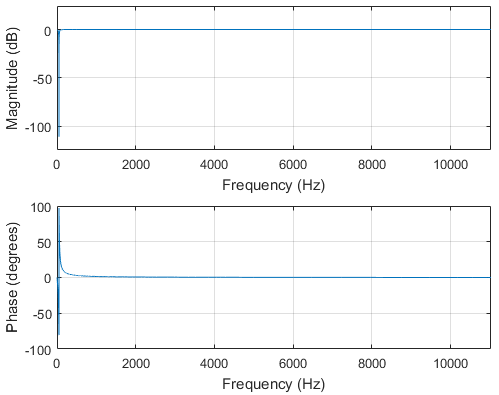
\includegraphics[scale=0.52]{Freqz_P-Z}  & 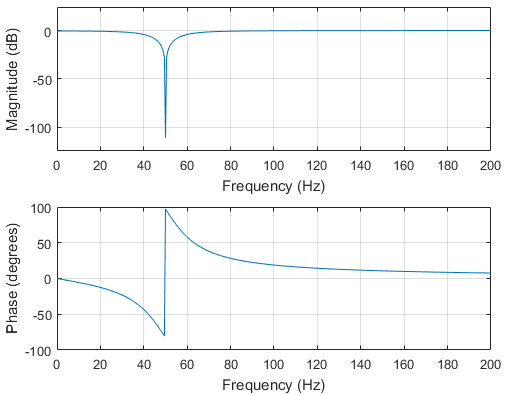
\includegraphics[scale=0.52]{Freqz_P-Z_zoom} 
\end{tabular}
\caption{Caption text here}
\label{tab:Reference}
\end{figure}
%%%%%%%%%%%%%%%%%%%%%%%%%%%%%%%%%%%%%%%%%%

%Labeled section
\section{Design}
\subsection{Frekvenser i et D}\label{subsec:FrekD}
%%%%%%%%%%%%%%%%%%%%%%%%%%%%%%%%%%%%%%%%%%

%Image from Matlab, using M-code to Latex
\begin{figure}[H]
    \centering
    \scalebox{0.45}{
    \input{Figurer/Blackman.pdf_tex}}
    \caption{Plot af et Blackmanvindue med 1201 samples}
    \label{fig:Blackman}
\end{figure}
%%%%%%%%%%%%%%%%%%%%%%%%%%%%%%%%%%%%%%%%%%

%Enumaration
Metode:
\begin{enumerate}
    \item Først bestemmes amplituden ved hver af fr diskrete frekvenser mellem 0 og Nyquist. Disse frekvenser findes ved følgende formel:
    \begin{equation}
       H_k \ @ \  \Omega_k = \frac{2\pi k}{2M+1},\ \ k = 0, 1, ..., M
    \end{equation}
    \item Herefter invers fourier transformeres disse ved brug af følgende forsimplede regneudtryk, som antager lineær fase:
    \begin{equation}
        b_n \ = \ h(n) \ = \ \frac{1}{2M+1}\bigg(H_0 + 2\sum\limits_{k=1}^M H_k \ cos\bigg(\frac{2\pi k(n-M)}{2M+1}\bigg)\bigg)
    \end{equation}
    \item Til sidst findes resten af filterkoeficienterne, som, grundet antagelsen om lineær fase, er magen til de beregnede, men spejlvendt (den sidste koefficient spejles dog ikke).
    \begin{equation}
        h(n) \ = h(2M-n), \ \ n=M+1,...,2M
    \end{equation}
\end{enumerate}
%%%%%%%%%%%%%%%%%%%%%%%%%%%%%%%%%%%%%%%%%%

%Table
\begin{center}
\begin{tabular}{| c | c | c |}
\hline
$F_s$ & Sampling frekvens & \SI{22.05}{\kilo\hertz}\tabularnewline
\hline
$F_c$ & Center frekvens & \SI{150}{\hertz}\tabularnewline
\hline
$BW$ & Båndbredde & \SI{50}{\hertz}\tabularnewline
\hline
\end{tabular}
\end{center}

%Using fixed cell sizes
\begin{center}
\begin{tabular}{||m{1cm}|m{1cm}|m{1cm}||}
\hline
    jasd & joke & lol\tabularnewline
    \multicolumn{3}{c}{Samlet tekst}\tabularnewline
    sokd & dsofksdof & sodfosd\tabularnewline
\hline
\end{tabular}
\end{center}
%%%%%%%%%%%%%%%%%%%%%%%%%%%%%%%%%%%%%%%%%%

%Code input using lstlisting package
%Part of a file
\lstinputlisting[firstline=1, lastline=3]{Matlab/kursus_opg_5_mads.m}

\lstinputlisting[firstline=20, lastline=30]{Matlab/kursus_opg_5_mads.m}

%Or entire file
\lstinputlisting{Matlab/Opg5_bandstop.m}
%%%%%%%%%%%%%%%%%%%%%%%%%%%%%%%%%%%%%%%%%%

